\chapter{Design and Implementation}
\newacronym{JSON}{$JSON$}{JavaScript Object Notation}
\glsadd{JSON}
\newacronym{TDS}{$TDS$}{Tabular Data Stream}
\glsadd{TDS}
\newacronym{MERN}{$MERN$}{MongoDB, Express, React JS, NodeJS}
\glsadd{MERN}
\newacronym{CORS}{$CORS$}{Cross-Origin Resource Sharing}
\glsadd{CORS}
\newacronym{MVC}{$MVC$}{Model-View-Controller}
\glsadd{MVC}
 
\label{requirements}
In the process of working on this project the functional and non-functional requirements of the system were identified and stated. This was formed through studying the literature and extracting the relevant details needed for the project. The functional requirements define how the system should work. The non-functional requirements specify the quality constraints that should be fulfilled. The functional requirements of the system are;
\begin{itemize}
\item Design a web server that gets attendance information from the database
\item The web server should render attendance information on the website
\item The web application should start the \gls{RFID} and fingerprint to track attendance
\item The web application should stop the \gls{RFID} and fingerprint, the web application should mark attendance with the following method and choice;
\item Mark attendance on entry only
\item Mark attendance on entry and exit
\item Mark attendance with fingerprint
\item Mark attendance with \gls{RFID}
\item Mark attendance with the manual method if there is a problem with the Raspberry Pi
\item A green LED response for a successful scan
\item A red LED response for an invalid scan
\item A blue LED response for an already scanned detail
\end{itemize}
while the non-functional requirements are:
\begin{itemize}
\item Flexibility: the system should use multiple methods to track attendance
\item The Raspberry Pi should handle unstable internet connection
\item The User Interface of the website should be minimised to enable components load quickly
\item The \gls{RFID} should be fast in scanning tags
\item The system should handle requests concurrently
\item The system is to be used at a fixed position. It would be best suited just outside the lecture room.
\end{itemize}

\section{Web Application}
\subsection*{Design \& Implementation}
In designing the monitoring system, a web application was decided because of its access from anywhere that has an internet connection. Each part of the system can access other systems connected to the internet.
For the web application, agile development cycle was used because the design and implementations of a software application is quite uncertain. Nonetheless, the use of this methodology had to do with the researcher's inexperience with this field. The iteration workflow involves the planning of requirements, developing the component, testing, iteration and feedback. The requirements were identified and stated\textsuperscript{\ref{requirements}} so as the specifications. After gaining an insight of the problem specification\textsuperscript{\ref{specification}} and its requirements, the languages and frameworks were considered. It was decided that a \gls{MERN} stack with an adaptation of Azure database as a database instead of MongoDB would be beneficial in development speed: the React, Express and Node apps are written in JavaScript. All components of the stack are open source. This allows a developer to get solutions to bugs and errors fast and effortlessly. Diving into the implementations made on the website, all pages have a dashboard that acts as a navigation bar to get to different web pages. The react application runs at localhost on port 3000 and the NodeJS server runs at localhost on port 8000. Based on the definition of same-origin or domain, their port number distinguishes them. This prevents them from communicating as a way to prevent cross-domain vulnerabilities like Cross-Site Request Forgery(CSRF). A \gls{CORS} extension is used for the communication between the website and nodeJS server by allowing one to perform cross-domain requests. This is done by adding Access-Control-Allow-Origin rule to the response header that was explained in the Background section. The \gls{MVC} architecture is used for developing the web application. It enables the application to be easily modified and scaled.
 
ReactJS serves as the view in the \gls{MVC} architecture, it allows the development of a websites user interface in JavaScript by rendering states on the \gls{DOM}. React often updates its state from a response obtained from the NodeJS server. The functions of the web pages included; a main page that shows a list of future events and a date picker or selector to pick an event to track. This was decided for development purposes. In  future this would be handled by the application and an event will be tracked based on the date. The attendance page was to handle the choices to track either \textit{mark only Entry} or \textit{mark both Entry and Exit}. Also \gls{RFID} and fingerprint buttons are designed to choose the method to track attendance. There is also a start and stop button and an analysis page that displays a datagrid on who was present and absent. However, the InProgress page was an afterthought. It was a concept designed after a couple of iterations that was meant to give details on certain constraints: A datagrid that showed students who were attending that event. However, a concept to display a list of people who scanned their attendance and refreshes every minute was initially considered but eventually discarded as it was thought to be quite distracting to the administrator while he is using the system for a different action.
Given that NodeJS is really good at handling simultaneous connections, it  is the controller in the \gls{MVC} architecture. \textit{attendanceController.js} handles the logic: converting database responses to valid data required by the view and handling requests from the view. In this project data is being sent and received from the database, the flask server and the front-end and sometimes concurrently and asynchronously. Furthermore, Tedious is a library that allows the implementation of TDS which is a protocol used to interact with SQL server. This enables the server to interact with the Azure database. Additionally, Express is used in this project to mount a middleware at the router-level. This allows one to handle multiple requests and responses to multiple end-points with one single mounted root path.
 
After a couple of iterations on the website, six pages were decided. While a manual attendance concept was schemed as another means to monitor attendance with the aim of providing a backup for failure in communication with the Raspberry Pi. A manual button was added to the attendance page. A student page was added to enable enrollment of \gls{RFID} and fingerprint details to the database although there was no impelementation.

\subsubsection*{Website}
\textbf{Main Page} - 
\begin{figure}[ht!]
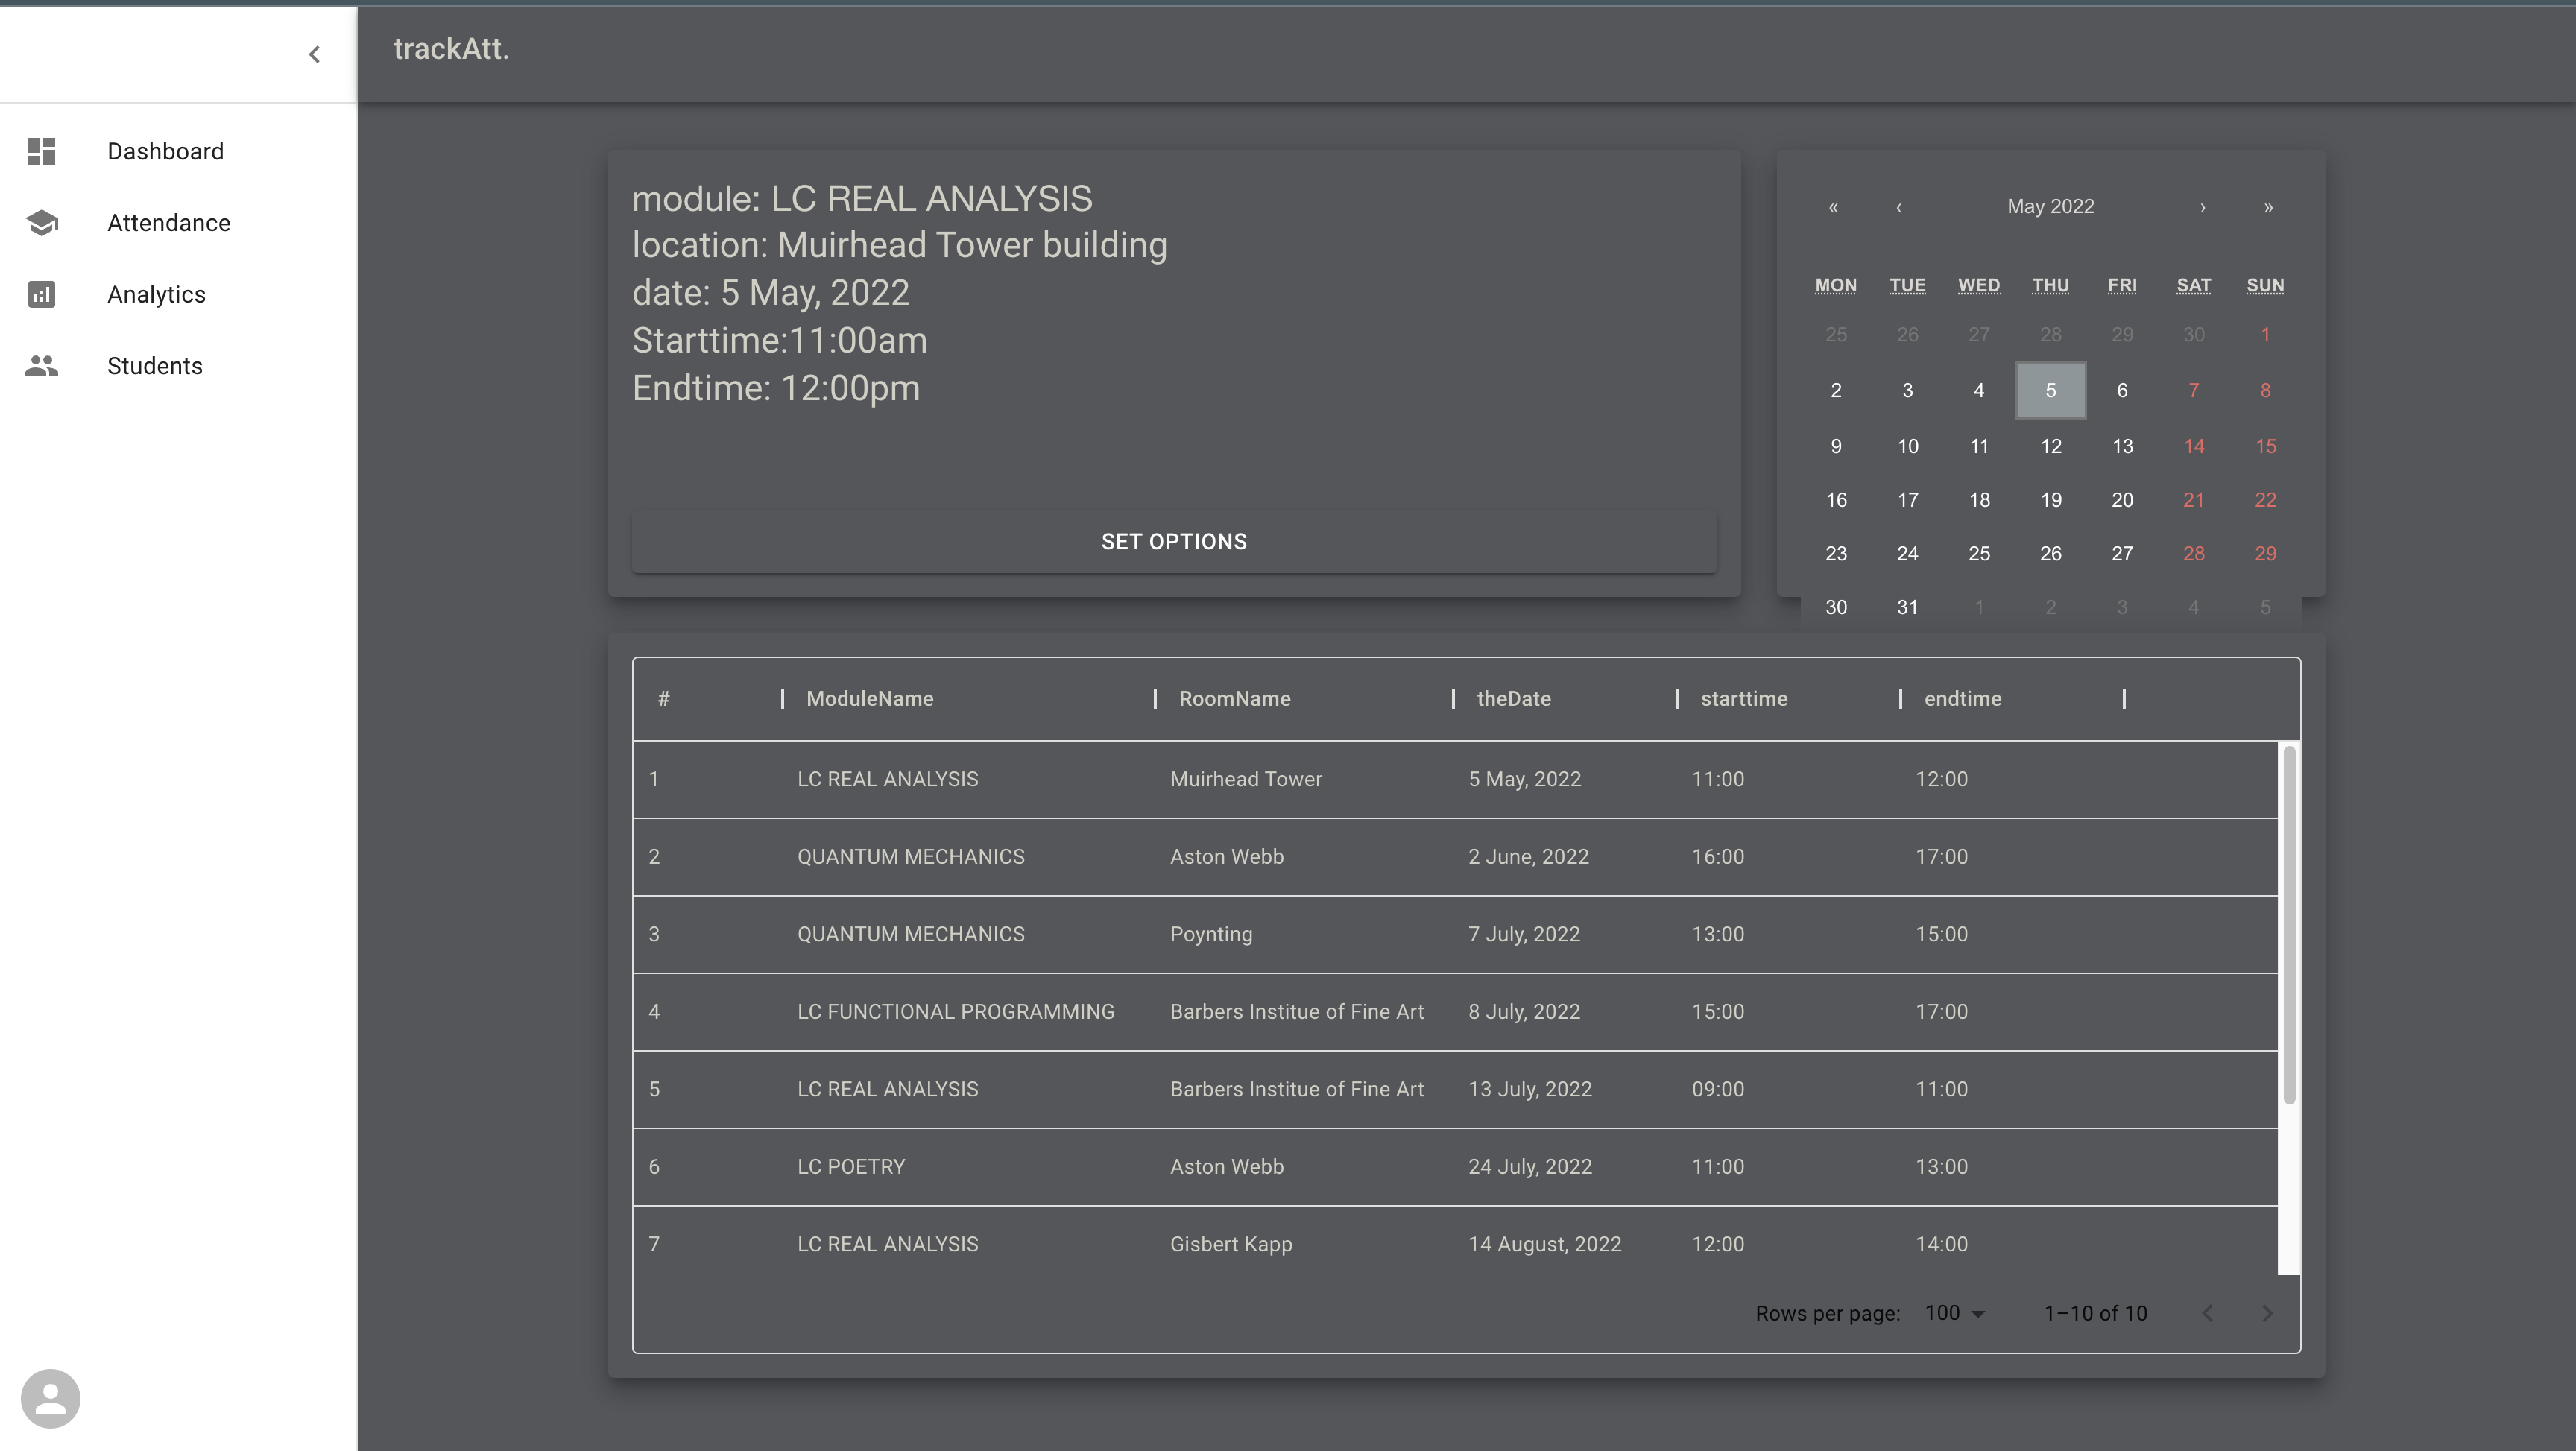
\includegraphics[scale=0.135]{Design & Implementation/images/Dashboard.png}
\caption{Dashboard/Main page.}
\end{figure}
The main page consists of the EventView at the top left, the CalendarView at the top right and the EventList at the bottom.The functions of these views are:
\begin{itemize}
\item CalendarView: The CalendarView is a date picker that selects the date and sends a request to the server for an event on that date. The default date is the current date at that moment.
\item EventView: The EventView displays an events information if there is an event on the date requested by the Calendar. It also has a "Set options" button that allows the administrator/lecturer to choose tracking methods and options by redirecting to the Attendance page.
\item EventList: The EventList displays a list of future events that the lecturer has.
\end{itemize}
Clicking the "trackAtt." logo takes you to the main page.

\textbf{Attendance page} - 
\begin{figure}[ht!]
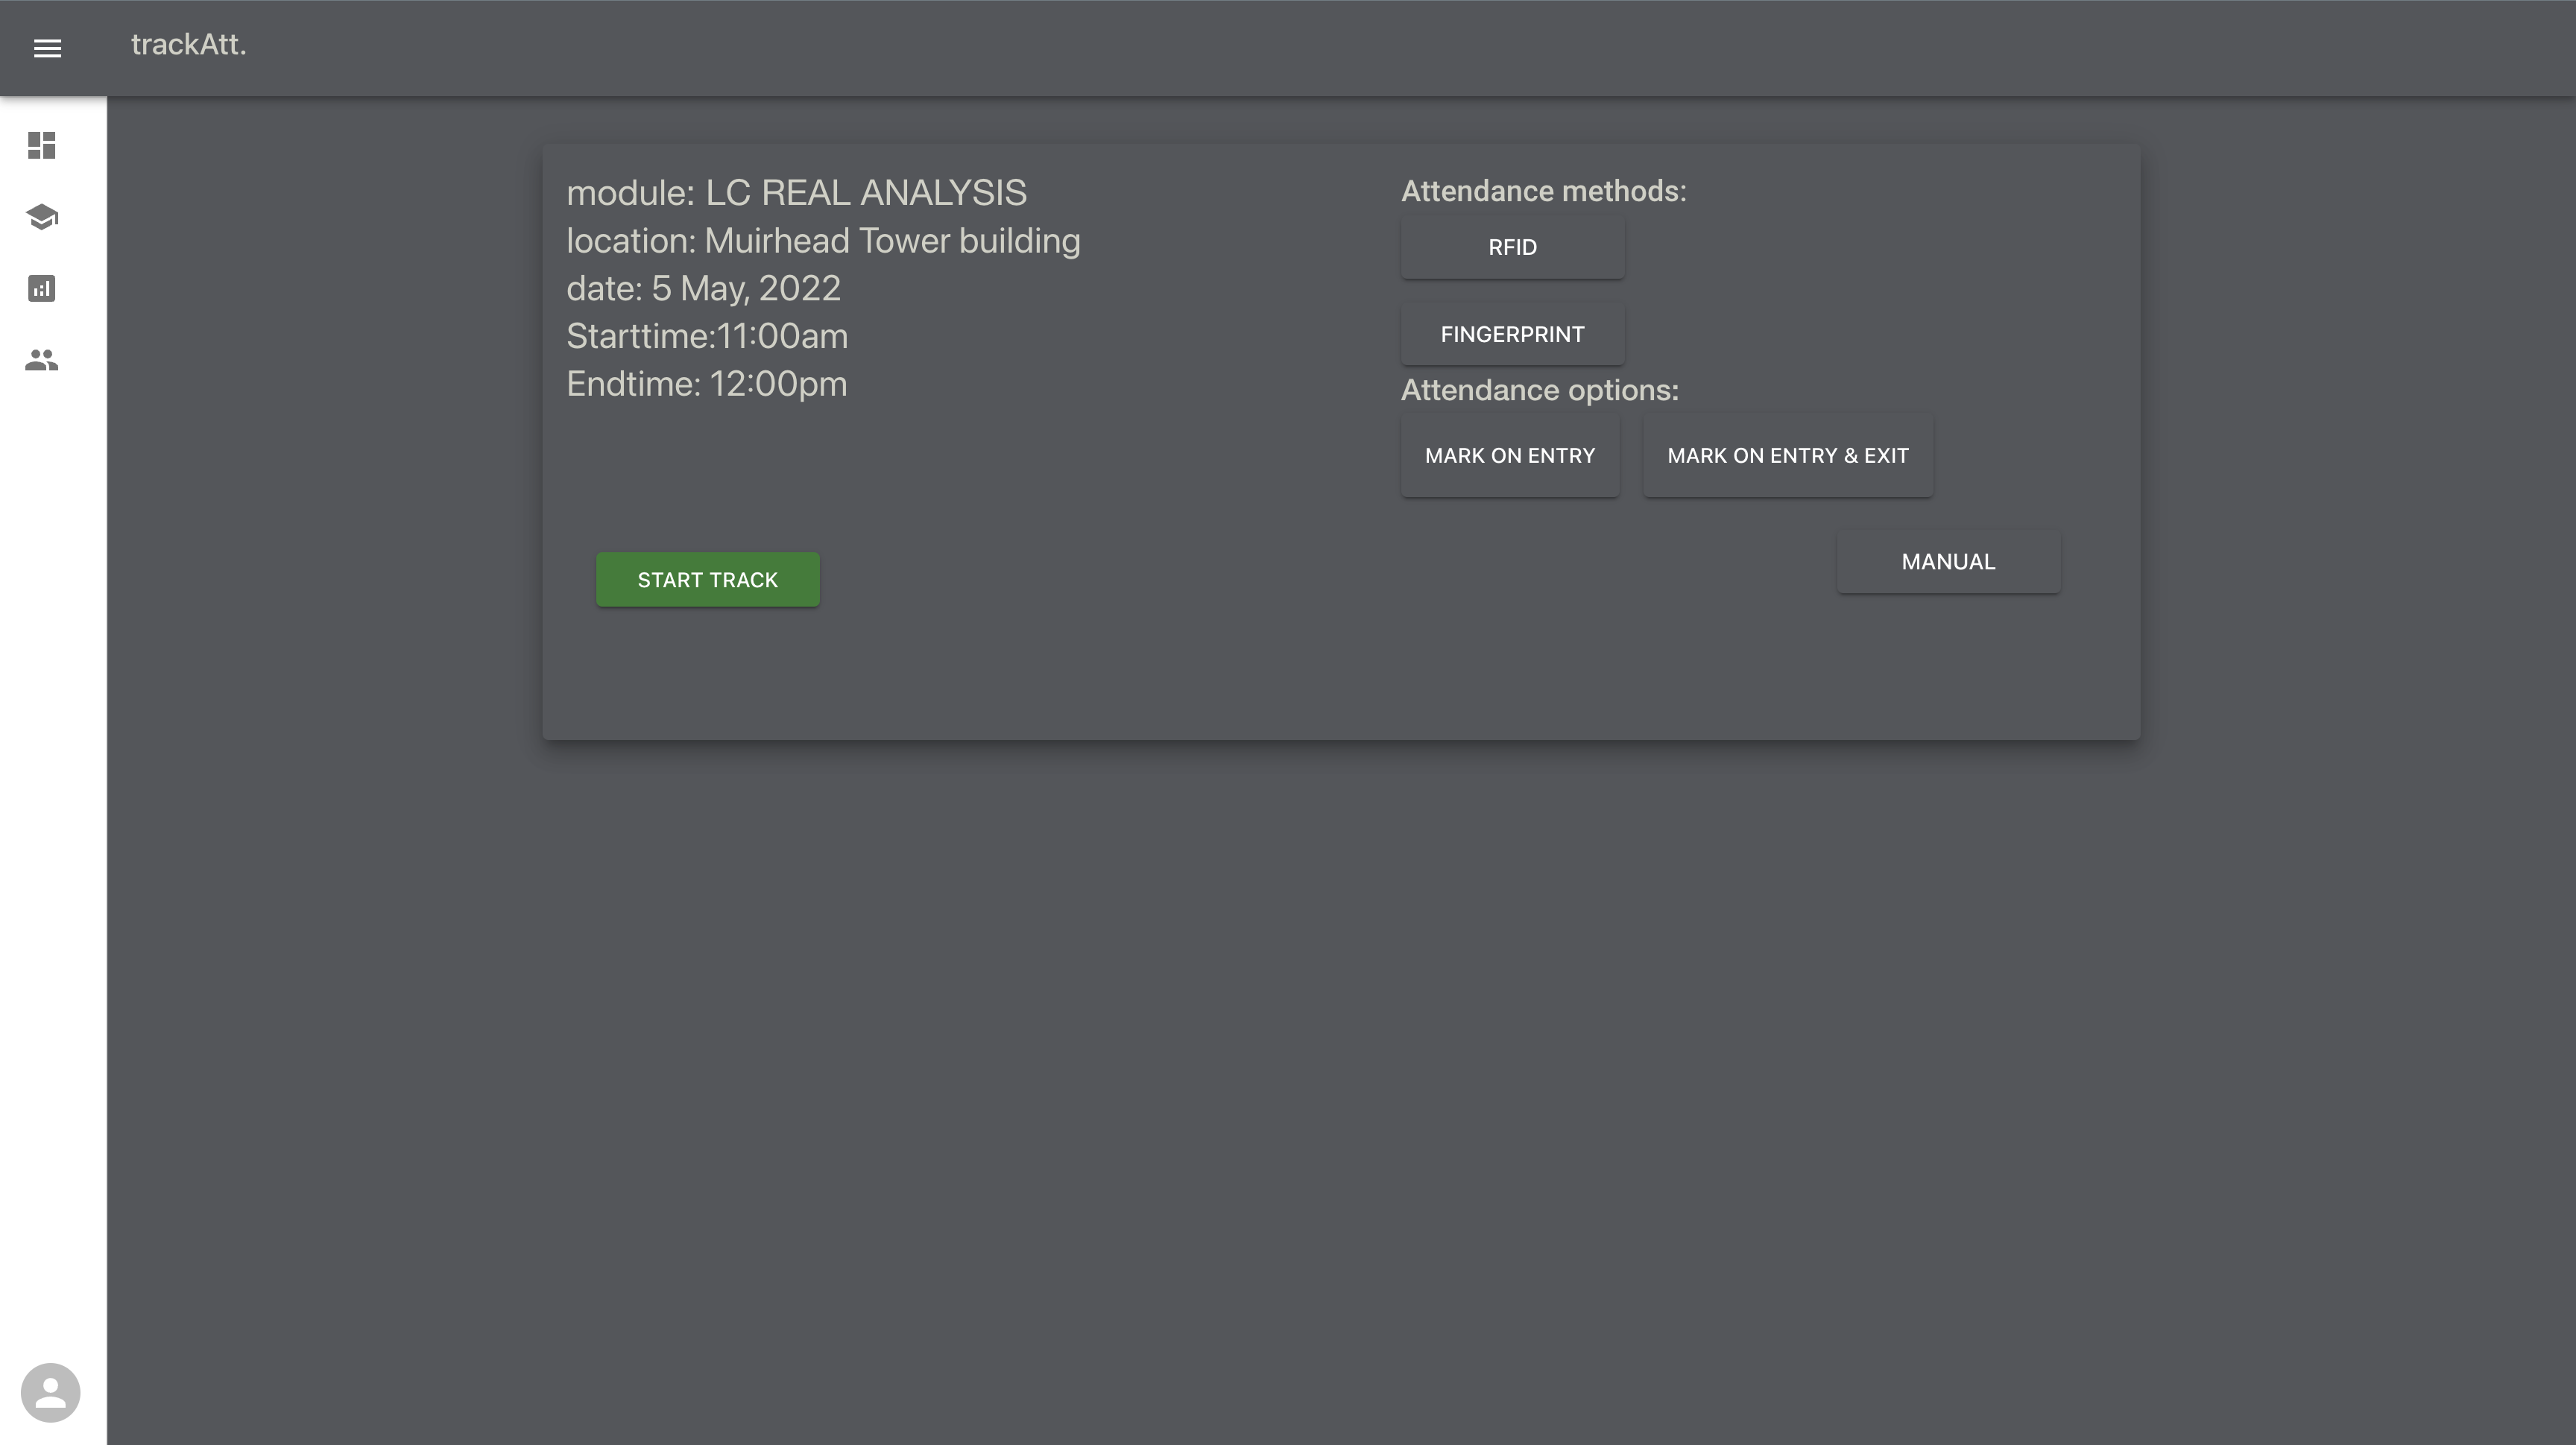
\includegraphics[scale=0.135]{Design & Implementation/images/Attendance.png}
\caption{Attendance page.}
\end{figure}
The attendance page is mainly accessed by the "Set options” button of the EventView. If directed to by the dashboard, it should show a list of events to track based on a date picker. However, this could not be developed due to time constraints. The main components of the Attendance page are the EventView but without a set options button, attendance methods with \gls{RFID} and fingerprint buttons, Attendance options with \textit{mark only Entry} and \textit{mark both Entry and Exit}, a \textit{Manual} button and a \textit{Start Track} button. The functions of these components are:
\begin{itemize}
\item EventView: The EventView displays information on the Event requested before by the CalendarView, gets a \gls{JSON} response from the server and formats the response to form the EventView details.
\item Attendance Methods: One method is chosen here. Either the Fingerprint method, the RFID method or the Manual method. Clicking on the fingerprint button sets the JM-101 module as the chosen method for tracking attendance while clicking on the RFID button sets the RC522 module as the chosen method for tracking attendance. The manual method is for a worst-case scenario where the Raspberry Pi can not track attendance and the teacher knowing each student by name can tick who is absent or present, clicking the button redirects to the Manual page.
\item Attendance Options: just like the Attendance Methods just one option can be used, clicking the "mark on entry" button sets the chosen tracking method to track only when the user scans at the beginning of the event while, "mark on both entry \& exit" requires the user to scan at the beginning and end of the event. These options were chose to model the flexibility of this system.
\item Start Track button: starts the tracking method with the attendance options chosen and also redirects to the "InProgress" page.
\end{itemize}

\textbf{InProgress page} - 
The InProgress page comprises a timer, a "Stop Track" button and a UserView that shows a list of Students that are required for that module.

\textbf{Analytics page} - 
The Analytics page contains the Attendance status of the event that was tracked and a pie chart diagram that shows the percentage of students who attended that session.

\textbf{Students page} - 
The Students page contains the whole list of students in the database.

\textbf{Manual page} - 
The Manual page displays a list of students. Each row has a checkbox that can be checked. If checked and submitted the students checked will be registered as present.
\subsubsection*{Web server}
The problem analysis in the Raspberry Pi explains the use of the nodeJS server in starting attendance. These are the major requests and responses handled by the express middleware;
\begin{itemize}
  \item receiveDate: a POST request that sets the date received from the client
  \item sendEvent: a GET request that runs a query to the database that gets all details of an event on a specific date and sends a \gls{JSON} response to the client
  \item sendEventList: a GET request that queries the database for a list of events which is sent to the client and displayed on the EventList
  \item startTrack: a POST request that gets an object which consists of the tracking method and option chosen. The object is sent as a POST request to the Flask server that runs a script to start the method chosen
  \item stopTrack: a POST request that checks the method running based on a global variable that was initially set when startTrack was called and sends a POST request to the Flask server endpoint to stop the process
  \item showAttendanceList: a POST request that queries the database for students taking a module based on a classID value that was already set for the current Event. This returns a response that sends a table containing who was present and absent(status)
  \item showAttendanceListWithoutStatus: a GET request that returns students taking a module based on a classID value
  \item showStudentList: a GET request that returns a list of students taking the current module that is being tracked
  \item showManualAttlist: a GET request similar to the showStudentList but the response is formatted in the front-end
  \item calculateAttendance: a GET request that returns the number of students who are present and absent. This is sent to the front-end and makes up the pie-chart in the Analytics page.
  \item addToAttManually: a POST request that adds users from an array obtained from the front-end.
\end{itemize}
 
\section{Raspberry pi}
\subsection*{Design \& Implementation}
The agile model was used for the development of the Raspberry pi system. The use of this methodology had to do with the researcher's inexperience with this field. An iteration cycle consisting the planning of requirements, developing the component, testing, iteration and feedback was used. In the requirement stage, questions were asked about the choice of components, languages, libraries and frameworks used. \textbf{Why the Raspberry pi?} for this project it was appropriate to use a microprocessor rather than a microcontroller. A microprocessor has a combination of prebuilt modules like a wifi chip, ethernet, bluetooth and other components. There is no need for external components although the necessary external components can be interfaced with the \gls{GPIO} pins. It is also capable of running multiple tasks simultaneously. This is a requirement of the system. A microcontroller like an Arduino uses a flash memory of 32KB. it would be impossible to store temporary database files that are required for the database exception handling because these are large data files with respect to the flash memory size whereas a Raspberry pi could use an SD Card with a much larger size. Additionally,
An \gls{RFID} is much more preferred because it identifies tags without direct line of sight in contrast with the Barcodes. It demonstrates a faster method of monitoring attendance compared to other tracking methods and would be suitable for a large number of students. \textbf{Why the Fingerprint?} The Fingerprint is a reliable means of monitoring attendance and represents a more secure option for a small set of people with a much more need for authenticity due to its unique use of fingerprints as stated in the Introduction. Most literatures that used this method used it because of its secure feature. Python was used for the development of the Raspberry Pi system because each method had a library developed in python.
A major reason why flask was decided is because it creates a local server in python and obviates the need to run python scripts in a different language or use an external framework. It is also a minimal framework and would be lightweight on the Raspberry pi making it have a much faster response when important scripts are created.
The MFRC522-python by mxgxw on github was initially used,\cite{mxgxwMFR34:online} but owing to some complications in its use, a switch to SimpleMFRC522 by pimylifeup was initiated because it was easy to adapt it to the required functionality.\cite{pimylife71:online}
Initially there was no response system to notify a tag or fingerprint had been scanned. After a couple of designs three LEDs were used: a green LED for when a tag has been scanned successfully, a blue LED for when a tag has already been scanned and red LED for when a tag is not recognized or is not in the module.
 
\subsection*{Problem Analysis}
\subsubsection*{Running python scripts}
From research it was initially reasoned that one could create python scripts for fingerprints and RFID modules to run. However, there was a problem getting the NodeJS server to run these scripts. The first method tried already had a loophole coming from the fact that the python script had to be on the same computer as the nodeJS server. Running it remotely from the Raspberry pi was also considered but the Raspberry pi did not give permission to run this script. Nevertheless, With further research it was observed that, using a local server on the Raspberry pi one could run a script from the server by creating a child process. This was perfect because it allowed one to encapsulate the scripts and access them only from the endpoints. This also sets the project up to run remotely as the NodeJS server can connect to it on the internet when the local server is hosted online.
 
\subsubsection*{Handling Database and Internet exceptions?}
Handling Database and internet exceptions is implemented in the attendance tracking scripts by catching a database or internet connection error by enclosing the connection codes in a try block:
\begin{verbatim}
try:
      conn = pyodbc.connect(driver=driver,
                            TDS_Version='8.0',
                            server=server,
                            port=1433,
                            database=database,
                            uid=username,
                            pwd=password)
      cursor = conn.cursor()
  except:
      readWithoutDatabase(moduleID, trackChoice, classID)
\end{verbatim}
This makes it easy to write another set of code which now performs a similar code function with respect to normal workflow if there was an internet connection. The internet handler is similar to the database handler. A way to check if there is a connection is by pinging a website. If there is any error with this it is caught in the try block\label{internet handler}:
\begin{verbatim}
try:
      urlopen('http://www.google.com', timeout=1)
  except:
      readWithoutDatabase(moduleID, trackChoice, classID)
\end{verbatim}
The offline code reads the scan of users into a csv file. Whenever the attendance system is used with a steady network connection the csv file is validated and converted into data that is uploaded to the Attendance column.
\subsubsection*{Using the fingerprint module to track students}
The fingerprint module stores read scans on the flash memory and validates based on that memory. Initially, the idea  of modifying the fingerprint to store templates on the Azure database with a BLOB type was considered. This however, was discarded due to time constraints and complexity in code: the \gls{API} code was shifting bits in the fingerprints to implement its functions. The position in flash memory of the student was stored in the database column "fingerprintID” whenever a student is enrolled. In an event where attendance is tracked the code checks the position of the user whose fingerprint has been scanned. The attendance scan is taken if a position exists. The implementation is explained further below\textsuperscript{\ref{fingerprint}}.
 
\subsubsection*{Scripts}
\begin{itemize}
\item \textit{RFID\_search.py}: The Script handles the RFID attendance tracking by first connecting to the database, then querying the database for a list of students who are intended for a particular module and stores the returned values in a global list variable. The script checks for the choice of tracking, if;
\begin{itemize}
  \item \textbf{markEntry}: Inside a while loop, an RFID reader function from the SimpleMFRC522 module. It tries to read a tag, when a tag is closeby. It gets the tags information and checks if the information is found in the database list. If it is found,it gets the studentID and stores this in the database table and on a counter so that it does not get inserted into the database, if it is scanned again.
  \item \textbf{markBoth}: inside a while loop, the RFID reader function tries to read a tag and waits for one to be closeby. If a tag is scanned it checks if it is in the database list. If it is in the database, it checks if that tag has already been scanned before by checking its counter value, if;
  \begin{itemize}
    \item \textbf{counter = 0}: an LED response with a green light, and the counter value is incremented by 1
    \item \textbf{counter = 1}: an LED response with a green light blinking twice, the counter value is incremented by one, the students RFID information are sent to the database
    \item \textbf{counter = 2}: a blue LED response to show that the tag has been scanned more than two times.
  \end{itemize}
\end{itemize}
An else statement if the RFID tag could not be recognized is used to show a status if the \textit{"if"} block case was not met. A red light LED response is used.
\item \textit{fingerprint\_search.py}: this handles the fingerprint attendance tracking by first connecting to the database. Then it initialises the fingerprint device. It queries the database for the fingerprint positions of students who are in the module. The scripts checks for the choice of tracking;
\begin{itemize}
  \item \textbf{markEntry}: A while loop similar to the \textit{RFID\_search.py} is used. Inside this the fingerprint module waits for a fingerprint. The right thumb is the finger used. When the right thumb has been read, a function from \textit{PyFingerprint} searches for a template that looks similar to the template read. This is the matching algorithm "1:N" discussed in the Background. The return value of this function is a position number which is an integer. It could be negative or positive. A negative number mainly "-1" implies that the position was not found while a positive number is its position in flash memory. A red LED response is witnessed if -1 is returned and it goes back to waiting for a template. Else the value is checked in the database list of students who are on the module list. If the student is found in the database list, a green LED response is witnessed and the students ID is added into the database. Else if the template has already been scanned a blue light response is shown.
   \item \textbf{markBoth}: Inside a while loop, the fingerprint module waits for a fingerprint. When one is recognised, it checks if it has a position in the flash memory. If not, it returns a red LED response and goes back to waiting mode. If it finds a position in memory, a check to see if that position has been scanned and added to the counter, if;
   \begin{itemize}
     \item \textbf{counter = 0}: the green LED response to show that it has been scanned, the counter is incremented by 1
     \item \textbf{counter = 1}: the green LED blinks twice to notify that fingerprint has been scanned twice
     \item \textbf{counter = 2}: the blue LED blinks to notify that the students attendance has already been taken.
   \end{itemize}
 \end{itemize}
 \item \textit{RFID\_enrollment.py}: this handles mapping an RFID tag to a student and storing it in the database. It connects to the database, and initialises the RFID module to read. The module waits for an RFID tag to scan. When an RFID is read, the write function gets the studentID of the student the tag is presumed to be mapped with and it generates an RFID \_UID\footnote{\label{RFID generation}by joining the first name, a random character from "A-Z", the last name and a random four-number string as a way to ensure security}. The tag details are inserted in the database row of that student.
 \item \textit{fingerprint\_enrollment.py}: this handles mapping the students to a fingerprint position that is stored in the database. The script connects to the database, it initialises the fingerprint module to read a fingerprint.\label{fingerprint} When a fingerprint is detected the \textit{searchTemplate} function checks for its position in memory to see if it has already been enrolled. If it has not been enrolled, the fingerprint is prompted to be removed and read again. This has to do with the algorithm "1:N" discussed in the background\textsuperscript{\ref{fingerprint 1:N}} comparing the two image characteristics of the fingerprint to form a template.
\end{itemize}
 
\subsubsection*{Flask}
These are the major requests and responses handled by the flask functions and endpoint.
\begin{itemize}
\item \textit{/RFIDread}: this is binded with the function \textit{readRFID()} which handles a POST request method. it expects three arguments from the web server as follows: the moduleID, the trackChoice and classID. A python process is invoked with \textit{Popen()} which runs the RFID python script \textit{RFID\_search.py} with the three arguments. The processID is stored globally to be used to stop the \gls{RFID}. A 200 response if everything works perfectly
\item \textit{/RFIDstop}: This is binded with the function \textit{stopRFID()} which handles a POST request method. It uses the global processID of the already started RFID python script to stop that process and also kills child processes that were spawned. A 200 response if everything works perfectly
\item \textit{/fingerprintread}: This is binded with the function \textit{readfingerprint()} which handles a POST request method. It expects three arguments from the nodeJS server; trackChoice, the moduleID and the classID. A python process is started which runs the fingerprint script \textit{fingerprint\_search.py} with the three arguments. The processID created when the process started, is stored globally. A 200 response when everything works perfectly
\item \textit{/fingerprintstop}: This is binded with the \textit{stopfingerprint()} function which handles a POST request method. No argument is expected. It uses the globally stored fingerprint processID variable to stop that process and any child process that was created and sends a 200 response if there is no exception.
\end{itemize}

\section{Database}
\subsection*{Design \& Implementation}
The AzureSQL database is the model in \gls{MVC} architecture. It stores the data required for the application to function. The database was complex because of the relationships between different tables. Thus 60\% of the designing time was spent updating it to fit other parts of the project. It needed  to be hosted on the internet in order to access it on multiple devices, Raspberry Pi and the development computer. At first a local MySQL database on my computer was used but there were issues with hosting this on the internet. Consequently, a switch to Azure was implemented because it offered several other cloud computing services. This was initially  a design of how the database would look like.
\begin{figure}[ht]
 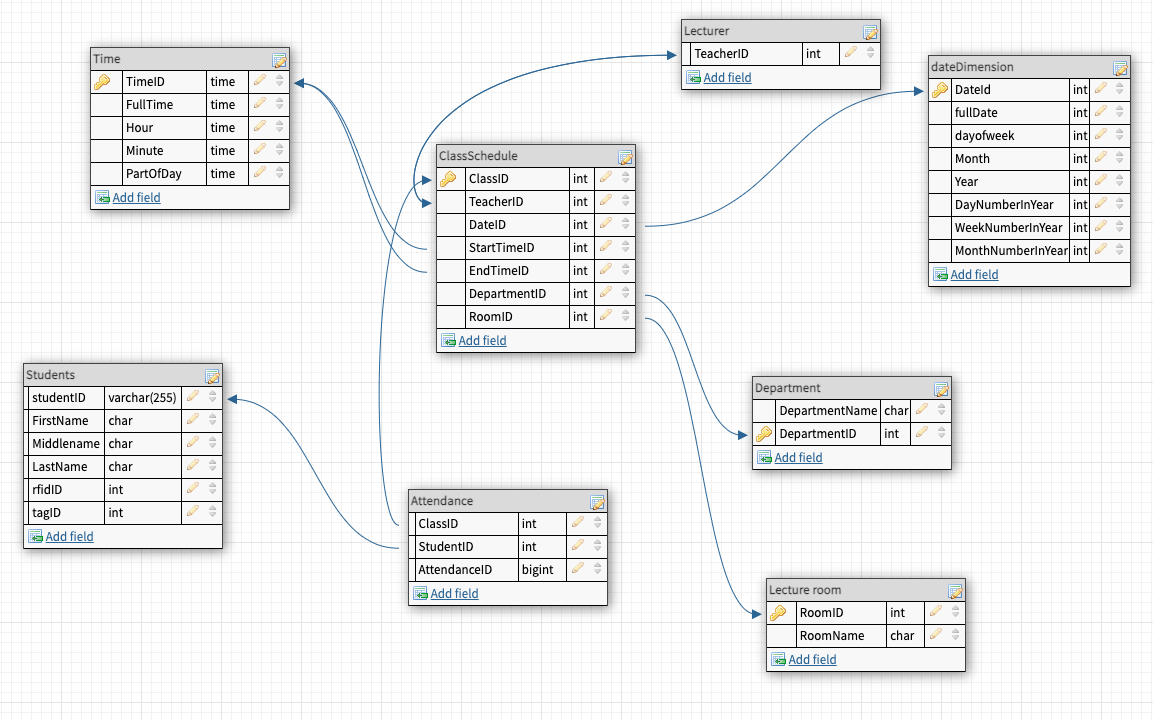
\includegraphics[scale=0.4]{Design & Implementation/images/database_design.png}
 \caption{database design}
 \label{fig:database_design.png}
\end{figure}
 
The design process of the database was similar to that of the web application, an agile development. In the requirement process, wireframe diagrams and pictures of each table and their functions were designed.  An example of this is figure\ref{fig:database_design.png}. After a couple of iterations of the agile cycle along with some testing with other systems, this was the structure of the database.
 
\begin{center}
 \begin{figure}[ht]
   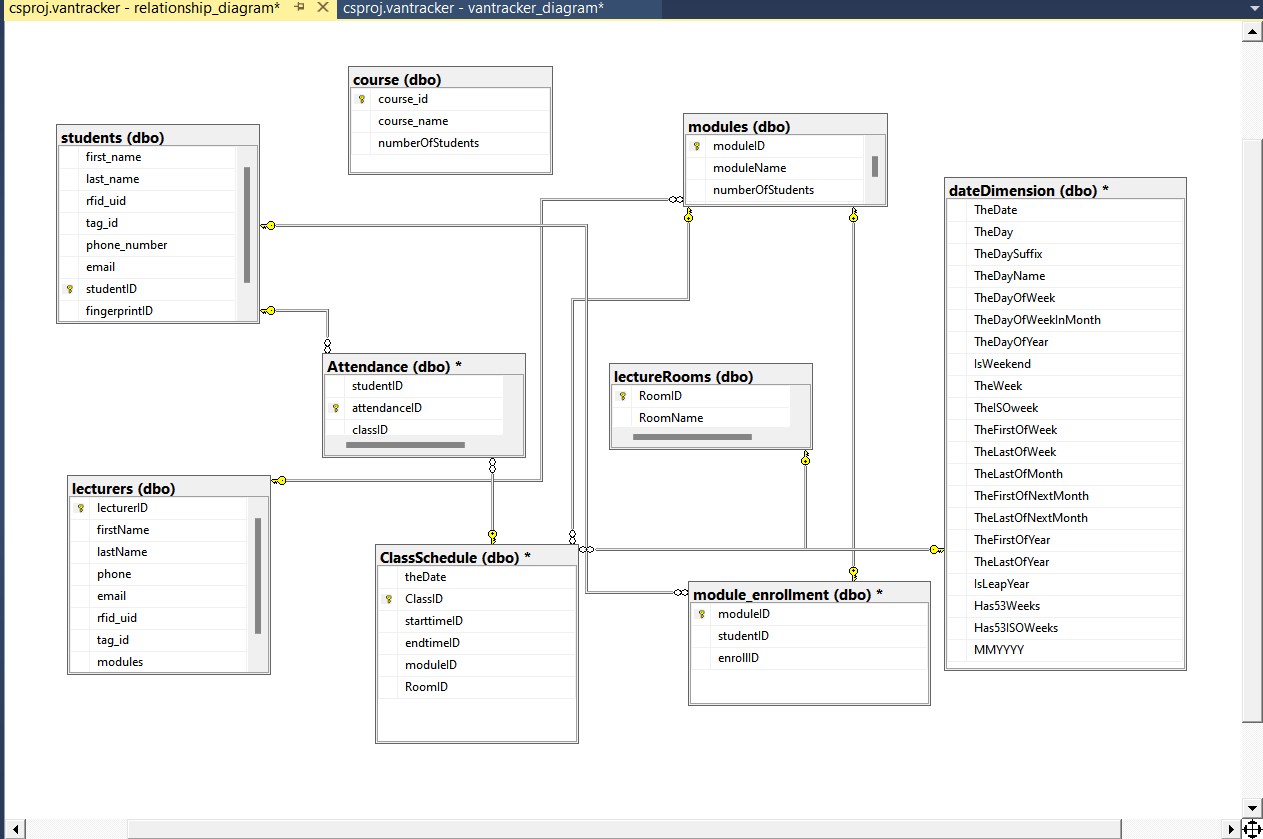
\includegraphics[scale=0.36]{Design & Implementation/images/2022-04-08.png}
   \caption{Implemented database design}
 \end{figure}
\end{center}
 
\subsubsection*{Time}
The time table was a representation of time. Following further research, this was deleted as it was found to be inefficient. It was quite redundant because making these columns a TIME variable worked better without the need to create a table for Time.
 
\subsubsection*{students}
For a student table, the first and last were split  name based. The studentID is the primary key and the rfid\_uid and tag\_id are the values obtained from the rfid tag The rfid\_uid is a random string generated in the \textit{rfid\_enrollment.py} which joins the first name, a random character from "A-Z", the last name and a random four-number string as a way to ensure security. The tag\_id is an immutable string that identifies the tag. These two fields are used to validate the rfid tags on the python scripts. The fingerprintID column contains the position of the fingerprint template stored in the fingerprint module memory. There is a phone number column and an email column also for identification and other implementations.
 
\subsubsection*{modules}
The modules table was created later, when designing a dummy dataset and trying to portray other entities that were not included in the database after several iterations of the workflow. The moduleID is the primary key, the numberOfstudents column keeps track of the number of students taking a module.
 
\subsubsection*{ClassSchedule}
The class schedule holds a record of every event that was held. The fields for this table are;
\begin{itemize}
 \item classID: The classID is the primary key of this table and is used to distinguish distinct classSchedule records
 \item TeacherID: used to identify a teacher or lecturer of the specific event. After several iterations this was refactored to lecturerID. There was no need for a lecturerID since the system does not implement any function that requires this field. This could be useful when the system works asynchronously for multiple lecturers.
 \item DateID: a foreign key with \textit{dateDimension} as its reference table. This allows access to other fields in the \textit{dateDimension} for another implementation
 \item Start and EndTimeID: To keep track of when the event takes place. This was initially designed to be a foreign key from the \textit{time} table.
 \item moduleID: a foreign key with a reference from the \textit{module} table, serves as a means to validate students who are intended for a specific class.
 \end{itemize}
 
\subsubsection*{dateDimension}
This functions as a customised calendar specifically designed for the University or organisation using the system. The dateID is the primary key, other fields were created in case of any other implementation. The column was referenced: it was created but not used in the implementation of the current system.
 
\subsubsection*{Lecturer}
This was designed to keep records of each lecturer in the database. A lecturerID as its primary key and a lecturerName.
 
\subsubsection*{Department}
The Department table had two fields. The departmentID which is the primary key and the departmentName. This was later found to be irrelevant to the scope of the project.
 
\subsubsection*{LectureRoom}
The lectureRoom table consists of a roomID which is its primary key and the Room Name. This is useful in keeping track of the location of the event.
 
\subsubsection*{course}
Represents the courses students took. It was designed to keep record of modules and students. The design of the relationship is quite complex and was irrelevant with the scope of the project.
 
 
\subsection*{Relationships}
A lectureRoom has a one-to-many relationship with a ClassSchedule because a ClassSchedule has one lectureRoom but a lectureRoom can be used for multiple ClassSchedule records. This is implemented by having a RoomID as a Foreign key in the ClassSchedule table with reference to the lectureRoom table. This is similar between the lecturer table and the ClassSchedule table although this was not implemented. A ClassSchedule has one lecturer but a lecturer record might have more than one ClassSchedule record. A ClassSchedule also has one module but a module might have more than one ClassSchedule record. This is implemented with the moduleID Foreign key in the ClassSchedule table. A many-to-many relationship is seen as a student can have multiple ClassSchedule records and a ClassSchedule can have multiple students. As stated in the Background,\textsuperscript{\ref{manytomany}} this is not supported in a Relational Database System but can be implemented by having a third table this table is the \textit{Attendance} table. This was used to store and validate attendance. The table consists of the studentID field and ClassID field. Another many-to-many can be seen between the student table and the module table. A \textit{module\_enrollment} table was designed for that relationship with the aim of validating students who were intended for a module. It contains a studentID field and a moduleID field. 
 
 
 
 
\section{System workflow}
 
\begin{figure}[ht]
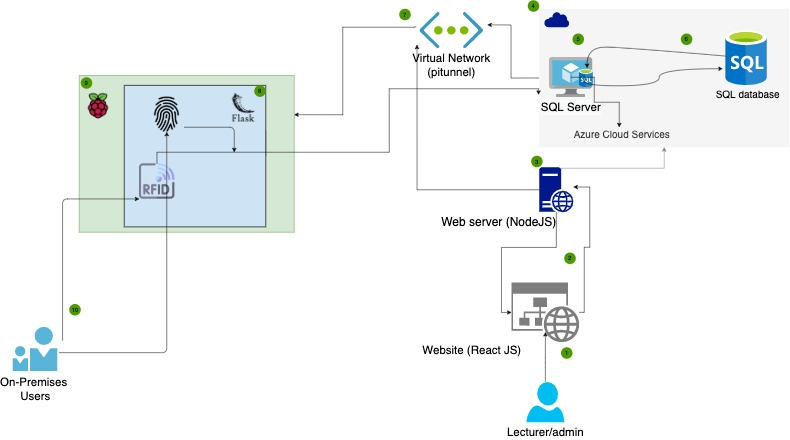
\includegraphics[scale=0.56]{Design & Implementation/images/system architecture.jpg}
\caption{System architecture}
\end{figure}
 
The administrator is first shown the MainPage. If there is an event on that day, the EventView shows them the Event details. They click on  the "Set Options" button and are redirected to the "Attendance Page". They chose the method to track and the option they would want and click on the Start button. If the manual button is clicked on the "Attendance page" they are redirected to the "Manual" page which shows a list they could tick based on who is present. The start button redirects them to the "InProgress" page which displays a timer along with a stop button. The Raspberry Pi system and the method is listening for a scan and would respond with the LED. A green response represents a successful scan. A blue response represents an already taken scan. A red response represents a user that is not available for the event or a scan that is not recognised. This leads to the evaluation of the system based on tests conducted.
